The HCal is the outer most part of the calorimeter and consists of two different detector technologies: the scintillating Title calorimeter (TileCal) in the barrel region, and the LAr based calorimeters in the end-caps\@.

The TileCal uses steel as the absorber material and plastic scintillator as the active medium. It covers the region $|\eta| < 1.7$ and is composed of a central barrel and two extended barrels, as shown in Figure~\ref{fig:atlas_calorimeter}. Between the central and extended barrels lies a gap region, which is instrumented with special steel-scintillator modules designed to partially recover energy lost in this area. Each barrel consists of 64 modules, each spanning approximately $\Delta\varphi = 0.1$. The modules are constructed with alternating layers of steel plates and scintillating tiles, with a volume ratio of about 4.7:1 in favor of steel. The absorbers provide approximately 7.4\intlength{}.

As hadrons traverse the absorber, they interact with nuclei in the material, initiating hadronic showers. These showers pass through the scintillating tiles, producing ultraviolet photons. The UV photons are then converted to visible light by special wavelength-shifting fibers, which transmit the photons to photomultiplier tubes (PMTs) for signal readout. A schematic of a TileCal module is shown in Figure~\ref{fig:atlas_hcal_module}.

\begin{figure}[htp]
    \centering
    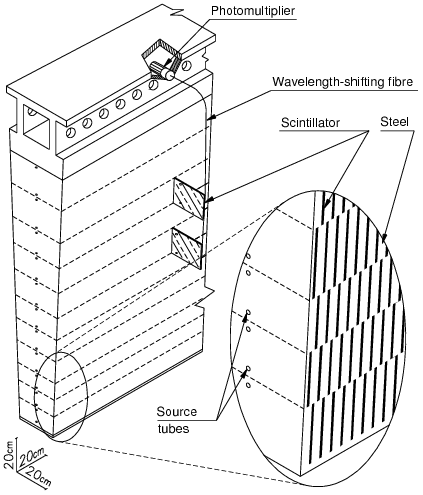
\includegraphics[width=0.5\textwidth]{figures/atlas/atlas_hcal_module.png}
    \caption{Schematic of a TileCal module illustrating the sampling structure of alternating steel absorbers and scintillating tiles. The optical readout system, including wavelength-shifting fibers and PMTs, is also shown. Taken from~\cite{atlas_collaboration_paper}.}\label{fig:atlas_hcal_module}
\end{figure}

The hadronic end-cap calorimeters (HEC) are a copper and liquid-argon sampling detector covering the range $1.5 < |\eta| < 3.2$. The HEC consists of two wheels in each end-cap with the front wheel (HEC1) and a rear wheel (HEC2) with each wheel consisting of 32 identical wedge-shaped modules. The modules in HEC1 consist of 24 copper plates with thickness 25 mm and a 12.5 mm thick front plate. The modules in HEC2 consist of 16 copper plates with thickness 50 mm, and front plate thickness of 25 mm. The gaps between the plates is where the active material, LAr, is located. These gaps have a thickness of 8.5 mm. The LAr gaps are further split by three electrodes creating four separate drift zones of 1.8 mm, and is shown in Figure~\ref{fig:atlas_hcal_endcap_module}.

\begin{figure}[htp]
    \centering
    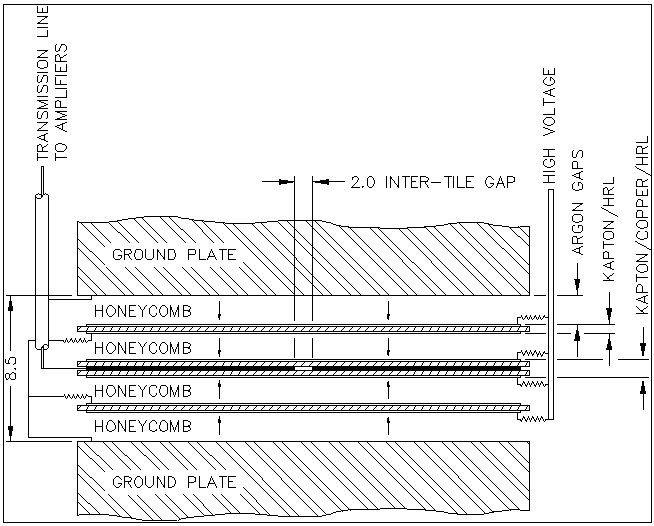
\includegraphics[width=0.7\textwidth]{figures/atlas/atlas_hcal_endcap_module.png}
    \caption{Schematic of a HEC module showing the LAr region between two copper absorber plates, subdivided into four drift zones by embedded electrodes. Taken from~\cite{atlas_collaboration_paper}.}\label{fig:atlas_hcal_endcap_module}
\end{figure}


